\documentclass[../statistical_learning_notes.tex]{subfiles}
\begin{document}
    %%%%%%%%%%%%%%%%%%%%%%%%%%%%%%%%%%%%%%%%%%%%%%%%%%%%%%%%%%%%%%%%%%%%%%%%%%%%%%%
    \chapter{Support Vector Machines}
    Maximal margin classifier is the first idea for the development towards SVMs. Maximal margin classifier utilizes hyperplanes and requires that the data is linearly separable. The extension of this is Support Vector Classifier that can be applied to an even broader class of problems where classes may not be perfectly separable. SVMs are a further extension of SVCs to account for non linear separation boundaries.

    \paragraph{Hyperplane} in a $p$-dimensional space is a surface that is an affine subspace (means it need not pass through origin) in the $p-1$ dimensional space. For a 2D space it will be a 1D line, for a 3D space it will be a 2D plane, and so on. The equation is of the form
    \begin{align*}
        \beta_{0} + \beta_{1}X_{1} + \beta_{2}X_{2} + \cdots + \beta_{p}X_{p} = 0
    \end{align*}
    Any point in the vector space can fall into one of the three regions
    \begin{align*}
        \beta_{0} + \beta_{1}X_{1} + \beta_{2}X_{2} + \cdots + \beta_{p}X_{p} \begin{cases}
            > 0\\
            = 0\\
            > 0
        \end{cases}
    \end{align*}
    and thus a hyperplane can be a useful demarcation between two regions or classes.\newline

    From now on, let $\beta^{T} = (\beta_{1}, \ldots, \beta_{p})$, $x^{T} = (x_{1}, \ldots, x_{p})$, $\beta_{0}$ be a scalar, and $N$ denote the total number of training data points. Although not represented by a bold font, $\beta$ and $x$ are both vectors. Since $\beta^{T}x$ is a scalar, $\beta^{T}x = x^{T}\beta$.
    

    %%%%%%%%%%%%%%%%%%%%%%%%%%%%%%%%%%%%%%%%%%%%%%%%%%%%%%%%
    \section{Maximal Margin Classifier}
    Maimum Margin Classifier uses hyper planes to find a separable boundary between linearly separable data points.\newline

    Suppose we have a set of data points with $p$ predictors and they belong to two classes given by $y_{i} = \{-1 , 1\}$. Suppose the points are perfectly separable through a hyperplane. Then the following hold
    \begin{alignat*}{2}
        &\beta_{0} + \beta^{T}x_{i} &&> 0 \quad \text{when} \quad y_{i} = -1\\
        \text{and} \quad &\beta_{0} + \beta^{T}x_{i} &&< 0 \quad \text{when} \quad y_{i} = 1\\
        \implies y_{i}(&\beta_{0} + \beta^{T}x_{i}) &&> 0
    \end{alignat*}

    Thus classification can be made into the positive or negative class simply based on the sign of the quantity $\beta^{T}x$. The further a point is, the more confident we will be in the classification.\newline

    Note that there can be infinite such hyperplanes that perfectly separate the data, and each can be obtained by slightly perturbing the given plane. Define margin as the minimum perpendicular distance from all training observations to this plane. The maximum margin classifier will be the one for which this margin is maximum.\newline

    \begin{figure}[h]
    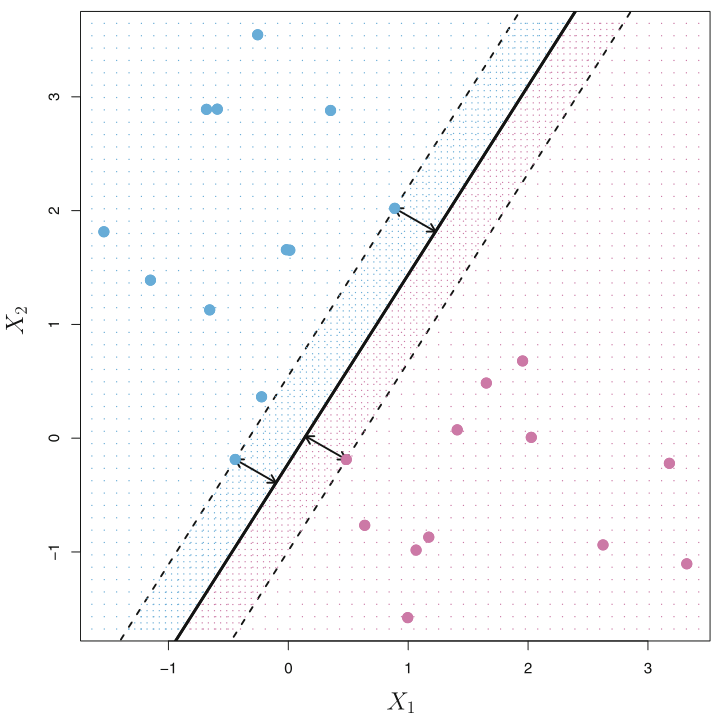
\includegraphics[scale=0.6]{mmc}
    \centering
    \caption{The Maximal Margin Classifier with the Support Vectors. Dotted lines represent the margin.}
    \label{fig:mmc} %\ref{fig:mmc}
    \end{figure}

    Note that the location of the maximal margin is determined only by the points closest to the boundary. If a point farther away would slightly move, the boundary would still be the same. Whereas if the point closer to the boundary would shift, the boundary itself would change as can be seen in figure \ref{fig:mmc}. These set of observations are know as \textbf{support vectors}. And by symmetry, the perpendicular distances of these closest points from the plane are same.

    
    %%%%%%%%%%%%%%%%%%%%%%%%%%%%%%%%%%%
    \subsection{Algorithm}
    Finding the boundary is same as solving for the following optimization problem ($M$ is the margin)
    \begin{align*}
        &\maximize_{\beta_{0}, \beta} M\\
        &\text{subject to} \quad \sum_{i=1}^{p} \beta_{i}^{2} = 1,\\
        &\text{and} \quad y_{i}(\beta_{0} + \beta^{T}x_{i}) \geq M \quad \forall \quad i = 1, 2, \ldots, N
    \end{align*}
    The constraint $\sum_{i=1}^{p} \beta_{i}^{2} = 1$ gives rise to the unique property that $\beta_{0} + \beta^{T}x$ is the perpendicular distance of the point $x$ from the hyperplane, making the last constraint equation valid. The proof of the perpendicular distance equation is given in section \ref{sec:appendix_mmc_perpendicular_dist}.\newline

    By using the perpendicular distance using the equation from section \ref{sec:appendix_mmc_perpendicular_dist}, we can replace the constraint on the norm and rewrite as
    \begin{gather*}
        \maximize_{\beta_{0}, \beta} M\\
        \text{subject to} \quad y_{i}(\beta_{0} + \beta^{T}x_{i}) \geq M \lVert \beta \rVert \quad \forall \quad i = 1, 2, \ldots, N
    \end{gather*}

    Note that the last equation remains same when we multiply by a positive constant. Hence, we can choose $\lVert \beta \rVert = 1/M$ for simplicity and the maximization problem becomes a minimization one (a factor of $1/2$ is introduced to simplify the derivative of the square term)
    \begin{gather*}
        \minimize_{\beta_{0}, \beta}  \frac{1}{2}\lVert \beta \rVert^{2}\\
        \text{subject to} 1 - \quad y_{i}(\beta_{0} + \beta^{T}x_{i}) \leq 0 \quad \forall \quad i = 1, 2, \ldots, N
    \end{gather*}

    For the following derivations involving linear optimization, refer to appendix (section \ref{sec:appendix_lagrangian}).\newline
    Invoking the Lagrangian multipliers, the new optimization problem is
    \begin{align*}
        \minimize_{\beta_{0},\beta}  \frac{1}{2}\lVert \beta \rVert^{2} - \sum_{j=1}^{N} \lambda_{j} (y_{j}(\beta_{0} + \beta^{T}x_{j}) - 1)
    \end{align*}

    where $\lambda = (\lambda_{1}, \ldots \lambda_{N})^{T}$. Using the Wolfe Dual, the following is the dual problem

    \begin{gather*}
        \maximize_{\beta, \beta_{0}, \lambda} L(\beta, \beta_{0}, \lambda) = \frac{1}{2}\lVert \beta \rVert^{2} - \sum_{j=1}^{N} \lambda_{j} (y_{j}(\beta_{0} + \beta^{T}x_{j}) - 1)\\
        \text{subject to} \quad \lambda > 0, \quad \frac{\partial L}{\partial \beta} = 0 \quad \text{and} \quad \frac{\partial L}{\partial \beta_{0}} = 0
    \end{gather*}

    The partial derivatives give
    \begin{align*}
        \beta = \sum_{j=1}^{N} \lambda_{j} y_{j}x_{j} \quad \text{and} \quad 0 = \sum_{j=1}^{N}\lambda_{j} y_{j}
    \end{align*}

    Substituiting in the dual,
    \begin{align*}
        L(\lambda) &= \frac{1}{2}\beta^{T} \beta - \sum_{j=1}^{N} \lambda_{j} (y_{j}(\beta_{0} + \beta^{T}x_{j}) - 1)\\
        &= \frac{1}{2}\beta^{T} \beta - \beta_{0}(\sum_{j=1}^{N} \lambda_{j} y_{j}) - \beta^{T}(\sum_{j=1}^{N} \lambda_{j} y_{j} x_{j}) + \sum_{j=1}^{N}\lambda_{j}\\
        &= \frac{1}{2}\beta^{T} \beta - \beta_{0}(0) - \beta^{T} \beta + \sum_{j=1}^{N}\lambda_{j}\\
        &= \sum_{j=1}^{N}\lambda_{j} - \frac{1}{2}\beta^{T} \beta
        = \sum_{j=1}^{N}\lambda_{j} - \frac{1}{2}(\sum_{i=1}^{N} \lambda_{i} y_{i}x_{i}^{T})(\sum_{j=1}^{N} \lambda_{j} y_{j}x_{j})\\
        &= \sum_{j=1}^{N}\lambda_{j} - \frac{1}{2} \sum_{i=1}^{N} \sum_{j=1}^{N} \lambda_{i} \lambda_{j} y_{i}y_{j}x_{i}^{T}x_{j}
    \end{align*}

    along with the constraints,
    \begin{gather*}
        \maximize_{\lambda} \sum_{j=1}^{N}\lambda_{j} - \frac{1}{2} \sum_{i=1}^{N} \sum_{j=1}^{N} \lambda_{i} \lambda_{j} y_{i}y_{j}x_{i}^{T}x_{j}\\
        \text{subject to} \quad \lambda > 0 \quad \text{and} \quad 0 = \sum_{j=1}^{N}\lambda_{j} y_{j}
    \end{gather*}

    which is a quadratic optimization problem with linear constraints, and is solvable through linear optimization softwares.\newline

    KKT conditions also need to be satisfied for the optimal solution, which gives
    \begin{gather*}
        \lambda_{j}^{*} (y_{j}(\beta_{0}^{*} + \beta^{*T}x_{j}) - 1 = 0 \quad \forall \: j = 1, 2, \ldots N\\
        \implies y_{j}(\beta_{0}^{*} + \beta^{*T}x_{j}) - 1 = 0 \quad \text{for points on margin}\\
        \lambda_{j}^{*} = 0 \quad \text{for points away from the margin}
    \end{gather*}
    which is expected based on the definition of the problem as only the points on margin decide the separating hyperplane. The predictions for new data points are simply made on the basis of the sign of $\beta_{0}^{*} + \beta^{*T}x$


    %%%%%%%%%%%%%%%%%%%%%%%%%%%%%%%%%%%%%%%%%%%%%%%%%%%%%%%%
    \section{Support Vector Classifier}
    The previous section was the best case scenario when all observations are perfectly separable. But in real data, this is seldom the case and we encounter the scenario that some observations will be misclassified. To take this into account, we maintain the same optimization as the previous section, but introduce new slack variables to account for the misclassified points
    \begin{align*}
        &\maximize_{\beta_{0},\ldots,\beta_{p}, M} M\\
        &\text{subject to} \quad \sum_{i=1}^{p} \beta_{i}^{2} = 1,\\
        &\text{and} \quad y_{i}(\beta_{0} + \beta_{1}x_{i1} + \cdots + \beta_{p}x_{ip}) \geq M(1-\epsilon_{i}) \quad \forall \quad i = 1, 2, \ldots, n\\
        &\epsilon_{i} > 0, \sum_{i=1}^{n}\epsilon_{i} \leq C
    \end{align*}

    which simply means that if
    \begin{enumerate}
        \item $\epsilon_{i} = 0$, we have correctly classified the observation
        \item $\epsilon_{i} < 1$, the observation is correctly classified, but lies between the hyperplane and the margin
        \item $\epsilon_{i} > 1$, the observation is misclassified
    \end{enumerate}
    
\end{document}